% ch03: 原文 GLDraft_D.tex 行 560–732；§2.3–2.4
% 只译散文（标题、正文、图题、脚注）；公式、\label、\ref、\eqref、\cite、图文件名保持不变。

 \subsection{希格斯丛模空间的量子化}\label{aphiggs}
 
 为了把这一构造用于某个规范群 $G$ 与黎曼曲面 $C$ 所对应的 $\M_H(G,C)$ 的量子化，我们真正需要研究的是它的四维版本。这意味着，要在 $\Sigma\times C$ 上研究规范群为 $G$ 的 $\N=4$ 超杨–米尔斯理论，其中 $\Sigma$ 是图 \ref{folding}(b) 中的长条。长条左、右两侧的边界条件，由 $\B_\cc$ 与 $\bB_\cc$ 的规范场论版本给出。$\B_\cc$ 在四维规范场论语言中的详细描述见 \cite{KW} 第 12.4 节。我们可以用一对 $(A,\phi)$ 来描述 $C$ 上的希格斯丛（Higgs bundle），其中 $A$ 是规范场，即 $G$-丛 $E\to C$ 上的一个联络\zy{原文作 $E\to G$，显系笔误——$G$ 是规范群，丛的底空间应是黎曼曲面 $C$；译文径改。}，$\phi$ 是取值于伴随丛（adjoint bundle）$\ad(E)$ 的 1-形式。在这一描述下，$\bB_\cc$ 由 $\B_\cc$ 经 $(A,\phi)\to (A,-\phi)$ 得到（并适当地延拓到四维超多重态的其他分量）。这是希格斯丛模空间上一个熟知的对合：它在复结构 $I$ 下全纯作用，在复结构 $J$ 与 $K$ 下反全纯作用。

尽管我们动用了规范场论与膜的机制，来构造与 $\M_H(G,C)$ 的量子化相联系的希尔伯特空间 $\H$，这一构造的实际产物却完全不令人意外。$\M_H(G,C)$ 中的一个稠密开集是余切丛 $T^*\M(G,C)$，其中 $\M$ 是 $C$ 上半稳定全纯 $G$-丛的模空间。几何量子化——或者干脆说初等量子力学——提示：与 $T^*\M(G,C)$ 的量子化相联系的希尔伯特空间，应当是 $\M(G,C)$ 上 $\lmark^2$ 半密度（half-density）的空间。

之所以要说 $\lmark^2$ 半密度而不说 $\lmark^2$ 函数，是因为在未选定某种测度\footnote{空间 $\M(G,C)$ 其实确有自然的测度，即把它视为 $C$ 上结构群为紧致群 $G$ 的平坦丛的模空间时，由其所携带的实辛结构给出的测度。这也是它嵌入超凯勒流形 $\M_H(G,C)$ 所诱导的测度。然而，这一测度并不属于 $A$-模型，也不会自然地出现在诸如希尔伯特空间 $\H$ 的定义这样的 $A$-模型构造中。}的一般光滑流形 $N$ 上，函数无从积分，因而没有自然的 $\lmark^2$ 函数的希尔伯特空间。流形 $N$ 上的一个密度是平凡实线丛 $\K$ 的一个截面，在任意坐标系中可局部写作 $|\d x^1\d x^2\cdots \d x^w| \,f(x^1,x^2,\cdots, x^w)$，其中 $f(x^1,\cdots, x^w)$ 是函数，而 $|\d x^1\d x^2\cdots \d x^w|$ 是测度，不是微分形式。$\K$ 有平方根 $\K^{1/2}$，它也是平凡的；其截面在给定坐标系中局部由函数 $g(x^1,x^2,\cdots, x^w)$ 描述，这些函数在坐标变换下的变换方式使得 $|\d x^1\d x^2\cdots \d x^w| \,g(x^1,x^2,\cdots, x^w)^2$ 不变。方便起见，把 $\K^{1/2}$ 的截面形式地写作
\be\label{formw} h=|\d x^1\d x^2\cdots \d x^w|^{1/2} g(x^1,x^2,\cdots, x^w)\ee
复值半密度由同一公式描述，只是局部 $g$ 取复值函数；它们以显然的方式构成希尔伯特空间：\be\label{ob} ||h||^2=\int |\d x^1\d x^2\cdots \d x^w|\, |g(x^1,x^2\cdots x^w)|^2.\ee
现在，出于将要应用于复流形 $\M(G,C)$ 的考虑，我们来描述复流形 $N$ 上的密度丛与半密度丛。若 $N$ 的复维数为 $n=w/2$，局部全纯坐标为 $z^1,z^2,\cdots, z^n$，则 $|\d z^1 \d z^2 \cdots \d z^n \d \bar z^1\d\bar z^2\cdots \d\bar z^n|$ 是 $N$ 上的一个密度，换言之是 $\K\to N$ 的一个截面。另一方面，$\d z^1 \d z^2 \cdots \d z^n $ 是全纯典范丛 $K\to N$ 的截面，而 $ \d \bar z^1\d\bar z^2\cdots \d\bar z^n$ 是复共轭线丛 $\bar K\to N$ 的截面（若给 $N$ 赋予相反的复结构，也可把它视为 $N$ 的典范线丛）。于是 $\K$ 可以等同于 $K\otimes \bar K$；更精确地说，$K\otimes \bar K\cong \K\otimes _\R\C$，即 $K\otimes \bar K$ 是复值密度丛 $\K$ 的复化。类似地，$K$ 至少在局部总有平方根；并且对 $K$ 的任一局部平方根的选取，都有 $\K^{1/2}\cong K^{1/2}\otimes \bar K{}^{1/2}$；更精确地说，$K^{1/2}\otimes \bar K^{1/2}\cong \K^{1/2}\otimes_\R \C$，即 $K^{1/2}\otimes \bar K^{1/2}$ 是复值半密度丛。只要 $\bar K{}^{1/2}$ 取作 $K^{1/2}$ 的复共轭，这一关系对 $K^{1/2}$ 的任意选取都成立。

在 \cite{GW} 第 3 节中，作者描述了这样的判别准则：$M=T^*N$ 的膜量子化（brane quantization），在赋予其余切丛的标准辛结构时，会导致 $N$ 上 $\lmark^2$ 半密度的希尔伯特空间。除了要求 $M=T^*N$ 有一个适合膜量子化的复化 $Y$ 之外，必要的条件是：$Y$ 应当是 $N$ 的某个复化 $W$ 的余切丛（并且 $Y$ 应具有余切丛自然的复辛结构）。若 $M$ 与 $N$ 本身已是复流形，而 $Y$ 定义为 $M$ 的两份拷贝之积、两份上赋予相反的复结构，则这一条件自动满足。

希格斯丛模空间 $\M_H(G,C)$ 以 $T^*\M(G,C)$ 为稠密开集，但它实际上并不同构于 $T^*\M(G,C)$。人们不会指望一个测度为零的差异会在 $\lmark^2$ 波函数的希尔伯特空间的定义中起重要作用。\cite{GW} 中的构造把量子化 $\M_H(G,C)$ 所得的希尔伯特空间 $\H$ 映到 $\M(G,C)$ 上的半密度空间，并不要求 $T^*\M(G,C)$ 恰好是整个 $\M_H(G,C)$。

$\M(G,C)$ 上半密度的希尔伯特空间 $\H$，早在 \cite{EFK} 中就已引入，那里完全没有提到膜、$\sigma$-模型或规范场论。通过膜的解释，才有可能运用电–磁对偶以及规范场论的其他方法。下一节讨论 Hitchin 哈密顿量时，我们会看到一个例子。


\subsection{Hitchin 哈密顿量}\label{hh}

如我们所见，在把一个复流形（例如 $\M_H(G,C)$）当作实辛流形来作膜量子化时，希尔伯特空间有一个展开（unfolded）的描述：$\H=\Hom(\bar\B_\cc,\B_\cc)$。$\H$ 承载\footnote{在折叠图像（folded picture）中，我们反而有代数 $\Hom(\B_{\cc,1},\B_{\cc,1})$ 与 $\Hom(\B_{\cc,2},\B_{\cc,2})$ 两者的左作用。一个代数的左作用，等同于其反代数的右作用。（反代数的概念在 \cite{GW} 的附录 C 中作了解释。）展开会逆转图 \ref{folding} 中一张叶片的定向，从而把两个代数之一换成其反代数。当然，哪个代数在左作用、哪个在右作用，取决于某些选取。这些在本文中都不重要，因为 $\A$ 与 $\b\A$ 将是交换的，从而同构于其反代数。} $\A=\Hom(\B_\cc,\B_\cc)$ 的左作用与 $\bar\A=\Hom(\bar\B_\cc,\bar\B_\cc)$ 的右作用。$\A$ 与 $\bar\A$ 分别是 $Y$ 上全纯函数所成交换环 $\A_0$ 与 $\bar\A_0$ 的量子形变。一般而言，形变所得的代数可以是非交换的；但在 $\M_H(G,C)$ 这一特殊情形中，$\A$ 与 $\bar\A$ 恰是交换的，因而左作用与右作用没有区别。


具体地说，在复结构 $I$ 下，$\M_H(G,C)$ 上全纯函数之环 $\A_0$ 就是 Hitchin 纤维化（Hitchin fibration）底空间上的函数环 \cite{H,NH}。考虑 Hitchin 方程的一个解 $(A,\phi)$，其中 $A$ 是 $G$-丛 $E\to C$ 上的联络，$\phi$ 是取值于 $\ad(E)$ 的 $1$-形式。令 $\varphi$ 为全纯希格斯场，即 $\phi$ 的 $(1,0)$ 部分。Hitchin 方程给出 $\bar\partial_A\varphi=0$。于是，若 $\P$ 是 $G_\C$ 的李代数 ${\g}_\C$ 上某个次数为 $s$ 的齐次不变多项式（invariant polynomial），则 $\P(\varphi)$ 是 $K_C^s$ 的全纯截面（$K_C$ 为 $C$ 的典范丛；我们还将记 $T_C=K_C^{-1}$）。给定 $C$ 上任一取值于 $T_C^{s-1}$ 的 $(0,1)$-形式 $\alpha$，可以定义
\be\label{juno} H_{\P,\alpha}=\int_C \alpha \,\P(\varphi). \ee
这是 $\M_H$ 上的全纯函数，且只依赖于 $\alpha$ 在 $H^1(C,T_C^{s-1})$ 中的上同调类。$H^1(C,T_C^{s-1})$ 的维数为 $(s+1)(g-1)$，这正是给定 $\P$ 时线性无关函数 $H_{\P,\alpha}$ 的个数。对 $G=\SU(2)$，$\M_H(G,C)$ 上全纯函数之环 $\A_0$ 由 $\P(\varphi)=\Tr\,\varphi^2$ 所对应的那些 $H_{\P,\alpha}$ 生成。更一般地，秩为 $r$ 的单李群 $G$ 有 $r$ 个独立的 Casimir 算子，对应 $r$ 个次数各异的齐次多项式 $\P_j$，$j=1,\cdots,r$，而 $\A_0$ 由 $H_{\P_j,\alpha_j}$ 生成。例如，若 $G=\SU(N)$，可取生成多项式为 $\Tr\,\varphi^{k}$，$k=2,3,\cdots,N$。

函数 $H_{\P_j,\alpha_j}$ 两两 泊松交换，因为 $\M_H(G,C)$ 在复结构 $I$ 下的全纯辛结构使得 $\varphi_z$ 与 $A_{\bar z}$ 成为共轭变量，特别地，任何只由 $\varphi$（而不含 $A$）构造的函数都两两 泊松交换。这些 泊松交换的函数就是 Hitchin 经典可积系统的哈密顿量。

\begin{yizhu}[译者按：Hitchin 纤维化与经典可积系统]
$\M_H$ 在复结构 $I$ 下是复辛流形，复维数为 $2\dim G\,(g-1)$；Hitchin 纤维化 $\M_H\to B$ 把希格斯丛映到其希格斯场的特征多项式（等价地，各次不变多项式 $\P_j(\varphi)$ 的取值），底空间 $B$ 是仿射空间 $\bigoplus_{j}H^0(C,K_C^{d_j})$，其中 $d_j$ 为 $G$ 各 Casimir 算子的次数，$\dim B=\dim G\,(g-1)$。原文说 $\A_0$ 是底空间上的函数环，意即 $\M_H$ 的整体全纯函数都来自底空间；这些 $H_{\P_j,\alpha_j}$ 两两 泊松交换，给出一个完全可积系统。对 $G=\SU(N)$，$B=\bigoplus_{s=2}^{N}H^0(C,K_C^{s})$，$\dim B=(N^2-1)(g-1)$。参见 Hitchin, ``The self-duality equations on a Riemann surface,'' Proc. London Math. Soc. {\bf 55} (1987) 59--126（即 \cite{H}），以及 ``Stable bundles and integrable systems,'' Duke Math. J. {\bf 54} (1987)（即 \cite{NH}）；亦见 \cite{BD}。
\end{yizhu}

从 $\A_0$ 到 $\A$ 的量子形变是无障碍的，意思是 $\A_0$ 的每个元素都可以量子形变到 $\A$ 的一个元素。具体地说，这句话意味着：若 $\P$ 是 $\g$ 上某个次数为 $s$ 的齐次不变多项式，$H_{\P,\alpha}$ 是对应的 Hitchin 哈密顿量，则存在一个微分算子 $D_{\P,\alpha}$，它作用在 $K^{1/2}\to \M(G,C)$ 的截面上，其主象征（leading symbol）等于 $H_{\P,\alpha}$。\zy{译者按（无外部依据）：$s$ 阶微分算子的主象征是其最高阶部分在余切丛上对应的函数，沿纤维为 $s$ 次齐次；对作用在半密度上的算子，它正是 $T^*\M(G,C)$ 上的函数，故可与 $H_{\P,\alpha}$ 相比较。}从 $H_{\P,\alpha}$ 到 $D_{\P,\alpha}$ 的过渡并不完全典范，因为指定 $D_{\P,\alpha}$ 所需的主象征之后，仍可给 $D_{\P,\alpha}$ 加上一个整体定义的低次全纯微分算子（次数小于 $s$）。对 $G_\C=\SL(2,\C)$，可取 $\P$ 的次数为 2，此时唯一整体定义的低次全纯微分算子就是 0 次算子——复常数。对秩更高的群，一般还有更多可能。在数学上，形变无障碍这一事实来自：对任何单群 $G$，$H^1(\M_H,\O)=0$，因此形变中没有潜在的障碍。这一论证的规范场论版本见附录 \ref{coho}，它细化了 \cite{KW} 中先前的讨论。

从 $\sigma$-模型或底层规范场论的角度看，从 $H_{\P,\alpha}$ 到 $D_{\P,\alpha}$ 的形变来自按 $\hbar$ 的幂次展开。这一展开在有限步之后终止，因为我们定义 $\A_0$ 由这样的函数组成：它们在余切丛的纤维上的限制是多项式。$\sigma$-模型或规范场论的具体定义给出从 $H_{\P,\alpha}$ 过渡到 $D_{\P,\alpha}$ 的具体处方，但这依赖于 $A$-模型并不包含的数据（例如 $C$ 上的黎曼度规，而不只是复结构）。

 \begin{figure}
 \begin{center}
   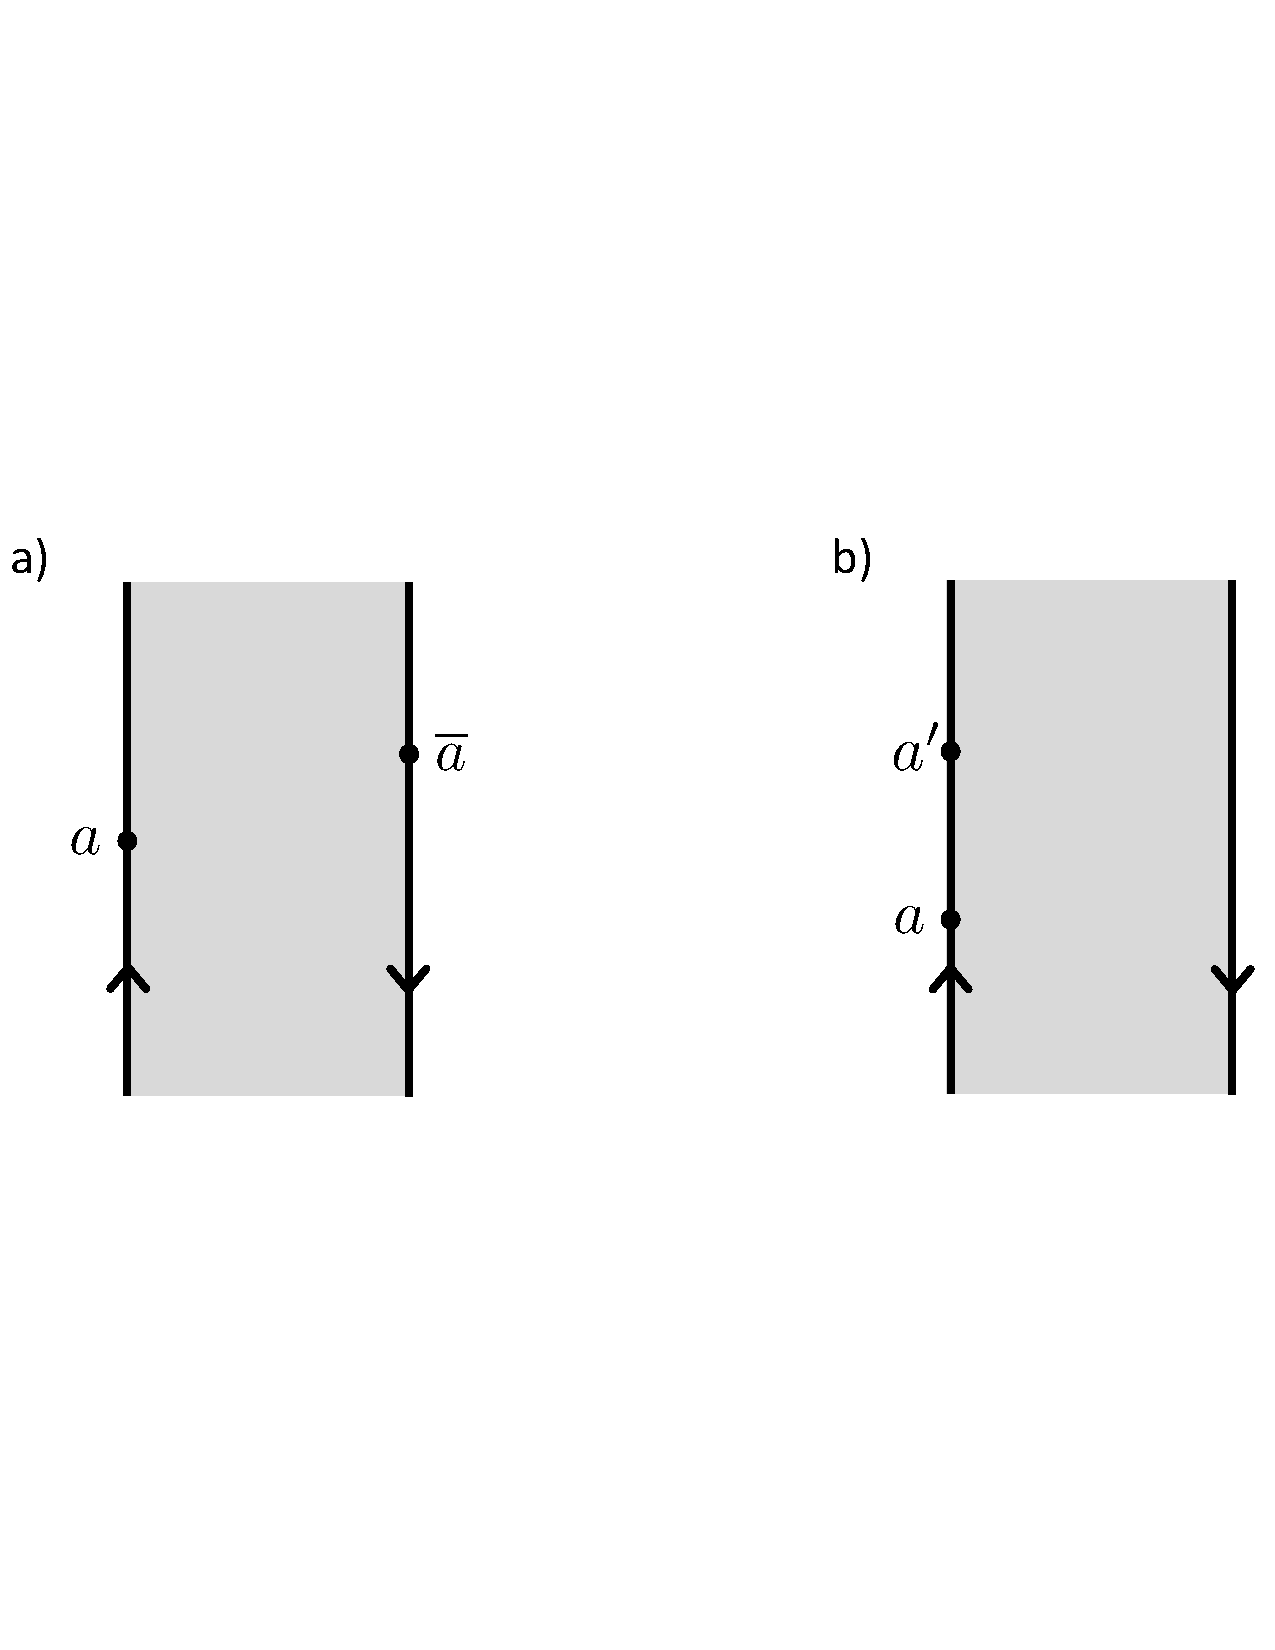
\includegraphics[width=4in]{Timing.pdf}
 \end{center}
\caption{\small (a) 作为二维拓扑场论中的一般性陈述，$\A=\Hom(\B_\cc,\B_\cc)$ 与 $\b\A=\Hom(\b\B_\cc,\b\B_\cc)$ 在作用于 $\H=\Hom(\b\B_\cc,\B_\cc)$ 时彼此交换，因为元素 $a\in\A$ 与 $\b a\in \b\A$ 被插入到相对的边界上。微分同胚不变性不允许任何关于谁“先”被插入的自然概念。(b) 一般而言，在二维拓扑场论中，$\A$（以及类似地 $\b\A$）可以是非交换的，因为元素 $a,a'\in\A$ 以相对于边界定向的确定次序被插入同一边界上。然而，在当前语境中还有两个额外的维度，即黎曼曲面 $C$，它们没有画在二维图像中。可以假定 $a$ 与 $a'$ 在 $C$ 中具有不相交的支集。因此，它们可以彼此上下错动而不出现奇点，故必须交换。\label{sliding}}
 \end{figure} 
 
接下来我们要解释为什么 $\A$ 像 $\A_0$ 一样是交换的。这最初由 Hitchin \cite{H2} 对 $\SU(2)$ 证明，并由 Beilinson 与 Drinfeld \cite{BD} 对一般单群 $G$ 证明。我们将给出一个类似于 \cite{KW} 中的四维解释。当然，同样的考虑也适用于 $\bar\A$。作为热身，先解释为什么 $\A$ 与 $\b\A$ 交换。这一点从以下事实即可看出（图 \ref{sliding}(a)）：元素 $a\in \A$ 插入在长条的左边界，而元素 $\bar a\in \b\A$ 插入在右边界。在二维拓扑场论中，我们可以沿边界独立地把这些插入上下滑动。两个边界插入之间没有有意义的相对时间序，因此它们必须交换。相比之下，考虑一对元素 $a,a'\in\A$ 的插入（图 \ref{sliding}(b)）。此时，作为二维拓扑场论中的一般性陈述，$a$ 与 $a'$ 之间存在有意义的时间序。若试图让其中之一在时间上滑过另一个，它们在交叉时可能出现不连续，因此一般而言可能有 $aa'\not=a'a$。然而，在当前问题中，我们其实不在二维而在四维；还有两个额外的维度构成黎曼曲面 $C$，它们未在图中画出。式 (\ref{juno}) 中 $H_{\P,\alpha}$ 的定义只依赖于 $\alpha$ 在 $H^1(C,T_C^{s-1})$ 中的上同调类。我们可以选取一个支集位于 $C$ 中任意选定的小开球内的代表元。因此，当我们考虑一对元素 $a,a'\in \A$ 时，可以假定它们由在 $C$ 中支集不相交的算子表示。于是，在图 \ref{sliding}(b) 的二维图像中，我们可以把这两个算子彼此上下错动而不出现任何奇点。因此它们交换。\zy{译者按：图内标题 “Diffemorphism inariance” 当为 “Diffeomorphism invariance” 之误（微分同胚不变性）。此系原文文字校勘，无外部依据；译文已按正名译出。}

我们可以稍加阐述量子 Hitchin 哈密顿量的四维起源。经典 Hitchin 哈密顿量中的被积函数 $\P(\varphi)$ 全纯地依赖于 $C$。正如我们在第 \ref{sec:chiral} 节所回顾的，量子 Hitchin 哈密顿量 $D_{\P,\alpha}$ 也可以写成 \be\label{qjuno} D_{\P,\alpha}=\int_C \alpha \,{\cal D}_{\P} \ee
其中 ${\cal D}_{\P}$ 是某些微分算子，它们在点 $p\in C$ 处局部地作用于丛上，并全纯地依赖于 $p$。我们把 ${\cal D}_{\P}(p)$ 认定为某个四维边界局部算符 $O_{\P}(p)$ 的作用。边界条件的全纯-拓扑（holomorphic–topological）性质保证：这类边界局部算符在拓扑方向上彼此交换，并且彼此之间的算子乘积展开（OPE）是非奇异的。

正如第 \ref{aphiggs} 节所解释的，量子希尔伯特空间 $\H=\Hom(\b\B_\cc,\B_\cc)$ 是 $\M(G,C)$ 上 $\lmark^2$ 半密度的空间，等价地，是 $K^{1/2}\otimes \bar K{}^{1/2}$ 的 $\lmark^2$ 截面的空间。我们回忆，之所以如此，是因为 $\M_H(G,C)$ 的膜量子化等价于把它作为余切丛 $T^*\M(G,C)$ 来量子化。在量子化余切丛 $T^*W$ 时，一个在余切丛纤维上的限制为 $s$ 次多项式的函数，会变成作用在 $W$ 上半密度上的 $s$ 次微分算子。若如当前所关心的情形那样 $W$ 是复流形，则更具体地说，$T^*W$ 上的全纯函数变成 $W$ 上的全纯微分算子。从全纯的观点看，人们通常说：$T^*W$ 上的全纯函数（对纤维为多项式依赖）变成作用在 $K^{1/2}$ 的截面上的全纯微分算子。（$K^{1/2}$ 的作用在 \cite{GW} 第 3.2 节与附录 C 中从 $\sigma$-模型的观点作了解释。）就 Hitchin 哈密顿量而言，它们可以被量子形变为作用在 $K^{1/2}$ 的截面上、而非任何其他全纯线丛的截面上的微分算子，这属于标准叙述的一部分 \cite{H2,BD}。然而，反全纯线丛 $\bar K{}^{1/2}$ 对于全纯微分算子是不可见的，因为它的转移函数是反全纯的，与全纯微分算子交换。因此，由 $T^*W$ 上全纯函数的形变量子化所得的全纯微分算子，自然地可以作用在 $K^{1/2}\otimes \bar K{}^{1/2}$ 上，等价地，作用在半密度丛 $\K^{1/2}$ 上。类似地，在形变量子化之下，$T^*W$ 上的反全纯函数变成作用在 $\K^{1/2}$ 上的反全纯微分算子。




 

于是 $\A$ 与 $\bA$ 分别成为作用在 $\M(G,C)$ 上半密度上的全纯与反全纯微分算子代数。从这个观点看，$\A$ 与 $\bA$ 交换这一陈述不过反映了全纯微分算子与反全纯微分算子交换这一事实。
